%!TEX root = ../main.tex
\documentclass[../main.tex]{subfiles}
\begin{document}
  \chapter{Method}\label{chapter:method}

  In this chapter we review the current methods for numerically solving partial-integro differential equations. We begin by considering the simplest model for the McKendrick-von Foerster Equation with constant coefficients and a simple first order approximation to solve it.

  To further this we consider the work of \cite{hartvig2011} who discuss a stable first order method for the McKendrick-von Foerster Equation when integral coefficients are used, but works equally well for constant coefficients. Finally, we discuss the boundary conditions and add the diffusion term to the problem.

  \section{First Order Upwind / Downwind Scheme}
  We first consider the McKendrick-von Foerster Equation with constant coefficients

  \begin{equation}
    L(u) = \frac{\partial u(t, w)}{\partial t} + g \frac{\partial u(t, w)}{\partial w} + \mu \cdot u(t, w)
  \end{equation}

  on the discretised domain $[0, T] \times [0, W]$. By simply replacing the time derivative with a forward difference and the spatial derivative with a backwards difference, we yield a first order approximation

  \begin{equation}
    D^n_j(u) = \frac{u^{n+1}_j - u^n}{h} + g \frac{u^n_{j} - u^n_{j-1}}{k} + \mu u^n_j.
  \end{equation}

  \subsection{Courant Condition} \label{method:sec:courant}
  At this point one might question the choice of the downwind scheme (backwards difference) as a choice for the spatial derivative. Ultimately this is for stability of the overall scheme. As discussed in \autoref{chapter:fdes} solutions to partial differential equations have an analytic domain of dependence. In \autoref{diff:fig:domainofdep} we saw the domain of dependence for the Advection Equation; due to the underlying structure the McKendrick-von Foerster Equation with constant coefficients inherits it shares the same domain of dependence.

  \cite{courant1928} researched the idea of a \emph{Courant Number}. In simple terms, the numerical domain of dependence (the region on which the numerical solution depends for information about its solution) must contain the analytic domain of dependence.

  Formally \cite{courant1928} stated that if the Courant Number

  \begin{equation}
    C = \frac{\upsilon \delta t}{\delta x} > C_{\mbox{\small max}},
  \end{equation}

  where $\upsilon$ is the largest magnitude of velocity that information travels in the system and $C_{\mbox{\small max}}$ is a constant that depends on the approximations used (normally $1$), then the finite difference approximation is unstable.

  \subsection{Stability of the Scheme}
  If we are to to solve the problem $L(u) = 0$ then we can rearrange $D^n_j$ to solve for $u^{n+1}_j$, which gives a recursive formula for $\mathbf{u}^n$:

  \begin{equation} \label{method:eq:mvffde}
    u^{n+1}_j = \left(1 + h \cdot \mu - \frac{gh}{k} \right) u^n_j + \frac{gh}{k} u^n_{j-1}.
  \end{equation}

  If we let $\lambda = gh k^{-1}$ then the matrix problem form of \autoref{method:eq:mvffde} is given by $\mathbf{u}^{n+1} = A \mathbf{u}^n$ where

  \begin{equation}\label{method:eq:noboundary}
    A = \begin{pmatrix}
      1 + h \cdot \mu - \lambda & 0 & \\
      \lambda & 1 + h \cdot \mu - \lambda & 0 \\
        & \lambda & \ddots & \ddots & \\
        &   & \ddots & 1 + h \cdot \mu - \lambda & 0 \\
        &   &        & \lambda & 1 + h \cdot \mu - \lambda
    \end{pmatrix}.
  \end{equation}

  Using the eigenvalue method we find the stability condition for this method is given by $k \leq g \mu^{-1}$.

  \subsection{Solution}
  To numerically solve the problems described in this chapter we will create an iPython notebook for each problem and produce a contour plot for each solution.

  \begin{figure}[htb]
    \centering
    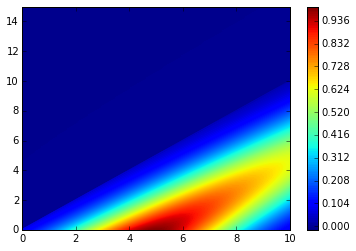
\includegraphics[width=0.5\textwidth]{_assets/advection_noPeriod.png}
    \caption{\label{method:fig:advectionPlotNoPeriod} Numerical solution of the Advection Equation with left boundary conditions unspecified. As expected we see that the initial condition decays along characteristic lines of the form $w - g t = C$ for $C \in \mathbb{R}$.}
  \end{figure}

  Using \autoref{method:eq:mvffde} as a model for iterating through each time step and using a Gaussian distribution as the initial condition we produce \autoref{method:fig:advectionPlotNoPeriod}. This shows a decreasing solution through time. However we note that above the line $w = gt$ the solution is zero, since there has been no specified left boundary condition. This is because the matrix $A$ in \autoref{method:eq:noboundary} does not appropriately deal with the derivatives in the boundary. On the left boundary for $w = 0$ we find that

  \begin{equation}
    u^{n+1}_0 = \left( 1 + h \cdot \mu - \lambda \right) u^n_0,
  \end{equation}

  which is clearly not an accurate approximation for $L(u)$. While plotting the numerical solution for this would, without further inspection, show that the left boundary is decreasing exponentially, which can be seen in \autoref{method:fig:boundayDepreciation}.

  \begin{figure}[htb]
    \centering
    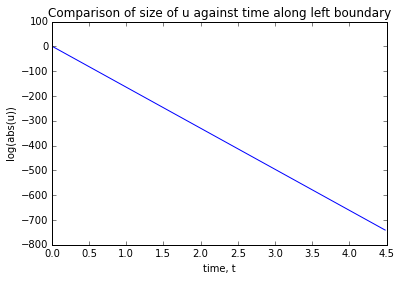
\includegraphics[width=0.5\textwidth]{_assets/uBoundary.png}
    \caption{\label{method:fig:boundayDepreciation} Logarithmic size of the solution to \autoref{method:fig:advectionPlotNoPeriod} along the left boundary $w = 0$.}
  \end{figure}

  To solve this issue and throughout the problems that follow, we imposed periodic boundary conditions on the domain so that

  \begin{equation}
    u(t, W_{\mathrm{Low}}) = u(t, W_{\mathrm{High}})
  \end{equation}

  for our choice of spatial domain $[W_{\mathrm{Low}}, W_{\mathrm{High}}]$. Biologically we can interpret this in terms of birth and death. On the boundary $w = 0$ the approximation considers the oldest individuals and the growth rate $g$ to determine the number of individuals who are born and have a weight less than the lower boundary of the domain. By taking $W_{\mathrm{low}} = k$ then we have that $u^n_{-1} = 0$ which is an appropriate birth weight. When we add this condition, the matrix $A$ is rewritten to include the extra term in the top right and

  \begin{equation}
    A = \begin{pmatrix}
      1 + h \cdot \mu - \lambda   & 0                         &         &                           & \lambda \\
      \lambda                     & 1 + h \cdot \mu - \lambda & 0       &\\
                                  & \lambda                   & \ddots  & \ddots                    & \\
                                  &                           & \ddots  & 1 + h \cdot \mu - \lambda & 0 \\
                                  &                           &         & \lambda                   & 1 + h \cdot \mu - \lambda
    \end{pmatrix}.
  \end{equation}

  A simulation confirms that the boundary conditions works. We see the solution decaying further over time and continuing to move to the right through the spatial domain for weight.

  \begin{figure}[htb]
    \centering
    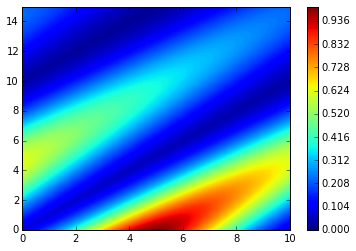
\includegraphics[width=0.5\textwidth]{_assets/advection_period.png}
    \caption{\label{method:fig:advectionPeriodic} The numerical solution of the McKendrick-von Foerster Equation with periodic boundary conditions. The solution continues decaying from the left boundary $w = 0$ when the solution carried along any characteristic meets the right boundary.}
  \end{figure}

  \section{Diffusion Term and Implicit Methods}
  Issues begin to arise when we consider the diffusion term within the upwind/downwind approximations.\autoref{method:fig:diffusionKChange} illustrates what happens for two different values of $k$ when we add the diffusion term using a second order downwind approximation.

  \begin{figure}[htb]
    \centering
    \subfloat[Solution $k$ = 2]{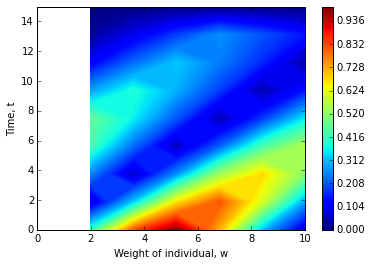
\includegraphics[width=0.45\textwidth]{_assets/diffusionLowK.png}}
    \subfloat[Solution $k$ = 0.4]{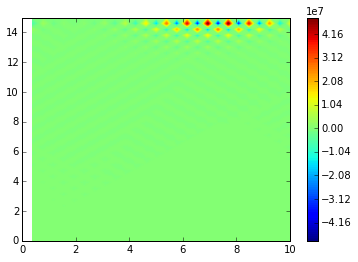
\includegraphics[width=0.45\textwidth]{_assets/diffusionHighK.png}}
    \caption{\label{method:fig:diffusionKChange} Comparison of the upwind/downwind scheme.}
  \end{figure}

  Even though the diffusion term should increase the analytic stability of the solution, we find that it increases the instability of the numerical approximations. To solve this we take a new approach, using implicit approximations instead of the explicit approximations.

  Instead of finding an equation for $u^{n+1}_j$ in terms of $u^n_i, i = ..., j-1, j, j+1, ... $ we aim to find an equation in the form $C \cdot \textbf{u}^{n+1} = c \cdot \textbf{u}^n$. If we begin to consider the McKendrick-von Foerster Equation with non-constant coefficients so that

  \begin{equation}
    L(u) = u_t + (g(w) \cdot u)_w + \mu(w) \cdot u.
  \end{equation}

  Using the approximation from \cite{hartvig2011}, which relies upon the semi-implicit derivative for products in \cite{press1992}, we can construct a first order implicit approximation

  \begin{equation}
    D^n_j(u) = \frac{u^n_j - u^{n-1}_j}{h} + \frac{g^{n-1}_j u^n_j - g^{n-1}_{j-1} u^n_{j-1}}{k} + \mu^{n-1}_j u^n_j.
  \end{equation}

  This method is stable under the assumption that $g, \mu$ are non-linear. However we note that the approximation for the derivative in weight is only first order. To look for a higher order method we consider the average of the forwards and backwards derivatives and add in the diffusion term to yield a finite difference equation

  \begin{equation}\label{method:eq:fullimplicit}
    D^n_j(u) = \frac{u^n_j - u^{n-1}_j}{h} + \frac{g^{n-1}_{j+1} u^n_{j+1} - g^{n-1}_{j-1} u^n_{j-1}}{2k} + \mu^{n-1}_j u^n_j - \frac{D^{n-1}_{j+1} u^n_{j+1} - 2 D^{n-1}_j u^n_j + D^{n-1}_{j-1} u^n_{j-1}}{k^2}.
  \end{equation}

  \begin{figure}[htb]
    \centering
    \subfloat[$\mu = 0.05$]{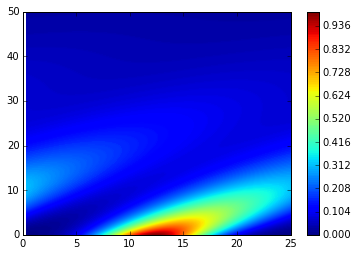
\includegraphics[width=0.5\textwidth]{_assets/diffusionSol.png}}
    \subfloat[$\mu = 0$]{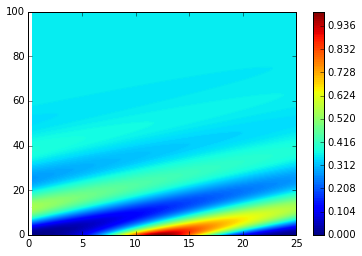
\includegraphics[width=0.5\textwidth]{_assets/diffusionSolNoDeath.png}}
    \caption{\label{method:fig:diffusionSolution} Comparison between values of $\mu$ for the McKendrick-von Foerster Equation with diffusion and periodic boundary conditions.}
  \end{figure}

  While the solution shown in \autoref{method:fig:diffusionSolution} shows that the scheme is stable, it still diffuses to a stationary distribution of $u_{\mathrm{stab}}(t, x) = 0$. However we note that the inclusion of the $\mu \cdot u$ term will kill the population over time, much like the solution of the McKendrick-von Foerster Equation without diffusion. Comparing this to the solution of the equation with $\mu = 0$ we see that the solution tends to a constant over time, closer to the solution that we aim to see in \autoref{chapter:modelequations}.

  \chapter{Discussion}

  In this project we have discussed the historical context of the McKendrick-von Foerster Equation and the Jump-Growth Equation and the numerical methods which are used when approaching similar problems. However we have not tried to apply these techniques to the McKendrick-von Foerster Equation with integral coefficients.

  \section{Integral Coefficients}
  If we consider modelling the integral coefficients using the approximation in \autoref{method:eq:fullimplicit} derived from the work of \cite{hartvig2011}, applying the same method used for the earlier results in \autoref{method:fig:diffusionSolution} with the implicit approximations from \autoref{method:eq:fullimplicit}, we can attempt to solve the equation numerically.

  Unfortunately, as \autoref{method:fig:integralCoefficientsFail} shows, the solution does not behave as expected using the same choice of parameters as Figure 2 \cite{datta2011}. While we do see the same decay as \autoref{method:fig:diffusionSolution}, the growth and diffusion terms do not have as much effect on the equation and thus the solution does not shift through the domain as much as the constant coefficient solution.

  \begin{figure}[htb]
    \centering
    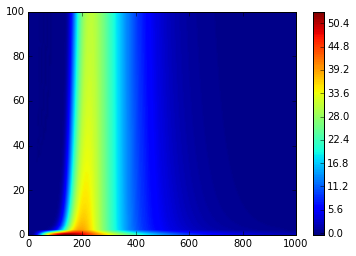
\includegraphics[width=0.5\textwidth]{_assets/integralCoeffsFail.png}
    \caption{\label{method:fig:integralCoefficientsFail} Numerical solution to the McKendrick-von Foerster Equation with integral coefficients. The solution diffuses slower than the McKendrick-von Foerster Equation with constant coefficients but still decays over time, though at a slower rate than the constant coefficient problem.}
  \end{figure}

  \section{Summary}

  While this project has not made direct advances on numerical methods for the various forms of the McKendrick-von Foerster Equation and its approximations to the Jump-Growth Equation, we have outlined a detailed framework for developing new methods from the existing methods and the work of \cite{hartvig2011}.

  Problems in partial differential equation theory do have numerical methods, but the study of the non-linear equations in this project is still in its infancy because methods are not developed thoroughly. Much of the research and time spent constructing our attempt at solving the McKendrick-von Foerster Equation with diffusion and non-linear coefficients has come from studying the problem with constants instead of functions and experimentation with approximations which are stable for those methods.

  \autoref{method:fig:diffusionKChange} and \autoref{method:fig:diffusionSolution} show that, while the diffusion term can greatly improve the stability of the solution to the equations, we will need to study the death term $\mu(w) \cdot u(t, w)$ if we are to avoid this dominating the derivative and making the finite difference equation converge to a $u(t, x) = 0$ steady state solution.

  Going forward, research will need to focus on dealing with the approximation error and stability in the integral coefficients, since it is clear from \autoref{method:fig:integralCoefficientsFail} that they are the root cause of the difficulty when studying the non-linear equations. As we saw in \autoref{chapter:fdes}, there is a large body of knowledge already developed around the approximation error and stability of finite difference equations and the same principles developed for approximating differentials can be applied to calculating integrals.

\end{document}
